% Author : Prakash Gautam
% Date   : 18-11-2019 13:06:42
%
\documentclass[a4paper]{article}

\usepackage{amsmath}
\usepackage{amssymb}
\usepackage{pgfplots}
\usepackage{fontenc}
\usepackage{physics}
\usepackage{graphicx}
\usepackage{tikz-feynman}
\usepackage{glossaries}
\usepackage{tikz}

\author{Prakash Gautam}
\input{EXOAcronyms.tex}

\begin{document}
    This is a demo
    \begin{align}
        ax ^2 + bx +c = 0
    \end{align}

    \begin{align*}
        x^{2} + bx = 0
    \end{align*}

    \begin{align*}
        ax^{2}
    \end{align*}
    
    \begin{align*}
        \Gamma(n) = \int\limits_{-\infty}^{\infty} e^{-x} x^{n}dx
    \end{align*}

    \begin{figure}[h!]
        \centering
        \input{0nbb.tex}
        \caption{}
        \label{fig:}
    \end{figure}
    
    This is a diagram for \gls{onbb}

    \begin{align*}
        \frac{x}{y}
    \end{align*}

    \begin{align*}
        \int\limits_{0}^{\pi} \frac{\sin{\phi}}{\cos{\phi}} d\phi
    \end{align*}

I can cite that \cite{prelovsekHeavyFlavorsLattice2017}
    \begin{figure}[h!]
        \centering
        % This file was created by tikzplotlib v0.8.5.
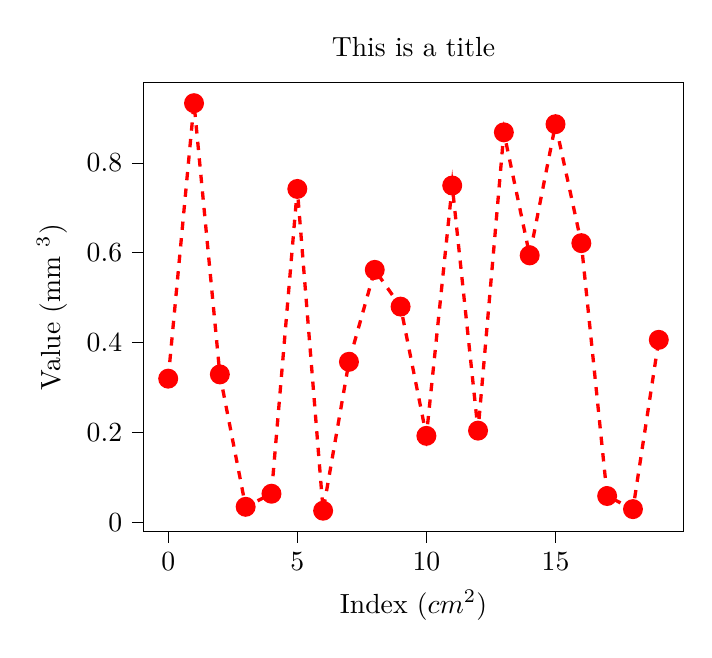
\begin{tikzpicture}

\begin{axis}[
tick align=outside,
tick pos=left,
title={This is a title},
x grid style={white!69.01960784313725!black},
xlabel={Index \(\displaystyle (cm^2)\)},
xmin=-0.95, xmax=19.95,
xtick style={color=black},
y grid style={white!69.01960784313725!black},
ylabel={Value (mm \(\displaystyle ^3\))},
ymin=-0.0195802058975972, ymax=0.978211906786268,
ytick style={color=black}
]
\addplot [very thick, red, dashed, mark=*, mark size=3, mark options={solid}]
table {%
0 0.319715861577799
1 0.932857719846092
2 0.329152998954912
3 0.0344631564100627
4 0.0635751468899814
5 0.741965834590709
6 0.0257739810425784
7 0.357167269053764
8 0.561845441503796
9 0.480032129481597
10 0.192419918403742
11 0.749596124410882
12 0.204038986152629
13 0.867951347189384
14 0.594042908573828
15 0.886070840023363
16 0.621322478472525
17 0.0584768111909409
18 0.0293375335828965
19 0.406124586885827
};
\end{axis}

\end{tikzpicture}

        \label{fig:}
    \end{figure}
     
    \bibliographystyle{ieeetr85}
    \bibliography{Femo.bib}
    
    


    
\end{document}
